\documentclass{article}


\usepackage{arxiv}

\usepackage[utf8]{inputenc} % allow utf-8 input
\usepackage[T1]{fontenc}    % use 8-bit T1 fonts
\usepackage{hyperref}       % hyperlinks
\usepackage{url}            % simple URL typesetting
\usepackage{booktabs}       % professional-quality tables
\usepackage{amsfonts}       % blackboard math symbols
\usepackage{nicefrac}       % compact symbols for 1/2, etc.
\usepackage{microtype}      % microtypography
\usepackage{lipsum}

\usepackage{graphicx}       %package to manage images
\graphicspath{{images/}}

\title{Compression in implementing digital pathology in network setting for mobile devices}

\author{
  Pargorn Puttapirat\thanks{Computer Science and Technology, Xi'an Jiaotong University, home page: \url{pargorn.puttapirat.com}} \\
  Department of Computer Science\\
  School of Electronic and Information Engineering\\
  Xi'an Jiaotong University\\
  Xi'an, China \\
  Student ID: 4119999057 \\
  \texttt{pargorn.puttapirat@g.swu.ac.th, pargorn@stu.xjtu.edu.cn} \\
}

\begin{document}
\maketitle

\begin{abstract}
This final project summarized two works which propose working architectures for supporting whole-slide images (WSIs) in digital pathology using globally accepted file format and communication standard (DICOM). The standard is generic thus can work on top of standard networking equipment and is readily available in hospitals around the world. Storing, retrieving, and viewing WSIs came with unique challenges due to their unusually large file size. In transition from conventional to digital pathology, the community will surely take advantage of practicing medicine remotely via mobile devices. To facilitate that, optimization for current technologies and conformation to standards is needed urgently. This work explore possibilities on method to reduce amount of file size and data transferring between servers and clients in pathology. We explore both lossy and lossless compression including new algorithm Guetzli for lossy JPEG compression and combination of generic PNG with ZLIB DEFLATE algorithm. The proposed computing scheme can work by leveraging the untapped power of processor and bandwidth between processors and memory units. By utilizing mentioned technique, we can reduce file size by approximately 30\% and 10\% in lossy and lossless compression. We also propose a scheme to decompress the file at the client therefore the amount of bandwidth needed could be reduced corresponding to compressed file size. 
\end{abstract}

\keywords{Digital pathology \and Whole-slide image \and Digital imaging and communication in medicine \ DICOM \and Computer network}

\section{Literature review}
Note: These two papers discuss on several topics beside wireless network and mobile computing. This summary will contain mainly the parts that are in the scope of this course. 

\subsection{Paper 1: An efficient architecture to support digital pathology in standard medical imaging repositories}
\paragraph{Citation:} \cite{marques_godinho_efficient_2017}
\paragraph{Key points}
\begin{itemize}
  \item In this paper, a web-based system that is fully compatible with DICOM standard is proposed. The system uses both DICOM file format and communication standard.
  \item The proposed architecture includes zero-footprint web-based viewer thus the clients were not required to have high processing power. This is good for mobile devices. 
  \item Performance of the proposed system which works based on DICOM-based file formats outperforms its counterpart which utilized proprietary formats. 
  \item DICOM-based data objects support storage of lossless files where proprietary file format does not. Yet, it still support partial access to the file which is crucial to accessing whole-slide images via wired/wireless networks. 
\end{itemize}

\paragraph{Background}
The goal of pathology has been the same for centuries despite the fact that the instruments that pathologists use, microscope, remains unchanged decades. Only recently (past decade) that there is a rapid development in pathology, transitioning conventional to digital pathology. This transition did not only include replacing glass slides to digital ones, but also include utilization of intelligent systems, applications in telemedicine or telepathology – making diagnosis remotely, longer-term file storage (glass slides cannot be kept for very long since they require a lot of environment-controlled physical space), more rapid access, and standardized viewer to view virtual slides accurately. 

The development of whole-slide imaging technology which can be used to digitized glass slides and produce digital slides known as whole-slide image (WSI). WSIs have enabled the field of pathology to take advantage of intelligent systems which has been rapidly developing in the past decade. WSIs are different from other general images since it contains a very high resolution, thus large in dimension, thus its introduction came with computational problems summarized in Table \ref{tab:table1}. 

\begin{table}
 \caption{Current requirements and solutions regarding whole-slide images}
  \centering
  \begin{tabular}{p{4cm} p{10cm}}
    \toprule
    \cmidrule(r){1-2}
    Characteristics of WSI     &  Solutions/work around to accommodate WSIs\\
    \midrule
    Large dimension and file size & Image tiling, cut the whole slide into tiles and store them as tiles (smaller image files).  \\
    Need for ability to view at low magnification. & Use pyramid scheme to save the image: Save the image as multi-resolution image including base layer where the bottom layer has the original resolution, then the upper layers have down-sampled version of the base layer. Therefore, when accessing the zoom-out view of the image, there is no need for the viewing algorithm to read the entire file which is very large and slow.  \\
    Need for partial accession or read.  & Tiling scheme can be used to support partial view by saving smaller tiles. After viewing requests are made, only relevant tiles can be read and stitched back together to construct the final viewing image. In DICOM servers, JPIP protocol allows viewer application to interact with JPEG2000 images over networks. \\ 
    \bottomrule
  \end{tabular}
  \label{tab:table1}
\end{table}

Beside the technical problems related to whole-slide imaging, there are problems regarding standards of WSIs as well. The idea of WSIs has been popularized in 1999, but DICOM standard has acknowledged the image type around 2011. This situation result in multiple proprietary file formats from different whole-slide scanner vendors and none of them is well-documented. The proprietary formats sometimes uses lossy compression and there is no way to access the original data, thus validation of original scans cannot be made. There are three main group of solutions to resolve this problem: (1) vendor neutral slide reading library such as OpenSlide library which is an open source library for reading majority of proprietary WSI formats; (2) convert whole slides into DICOM file format (or “DICOMize”), while there are several tools to perform this, clinical records and associated metadata in the generated DICOM files would have gone missing; (3) encourage whole-slide scanner vendors to adopt general DICOM standard and produce DICOM files from their scanner in the first place. This method is preferable and DICOM files would be compatible with DICOM server thus digital slide files can be stored on existing medical infrastructure. 

There are two attempts to develop DICOM-based protocol for accessing WSIs via content delivery and retrieval scheme. First is via SOAP protocol but it is considered to be heavyweight technology, therefore not suitable for web-services. Later, proposal of RESTful APIs was made to develop DICOM-web standard as a new and modern protocol to access resources on DICOM servers. 

In this paper, the authors propose architecture to implement digital pathology including slide storage and viewing based on general standard, DICOM, with purely web technologies, thus being open source solution. The proposed system will be tested against similar system that uses proprietary file formats. Performance of the two system will be tested on image visualization response time and processing capacity. 

\paragraph{Method}
First, establish the proposed architecture consist of DICOM files generation with existing WSIs, then setup a DICOM server as the first environment for performance testing experiment. Second, setup another environment using proprietary file format for storage and accession. Finally, perform visualization testing by opening images and perform simulated zooming and panning actions. Response time and processing capacity were recorded as performance of each system. 

\paragraph{Result}
The dataset of one hundred WSIs was used. In the dataset, the largest WSI has a file size of 19.4 GB with dimension of 26 Giga-pixels while the smallest has dimension of 16 Mega-pixels. The proposed architecture can perform 18 times faster than its counterpart, completing all tasks in less than 2 seconds. Each image tile was loaded in 20 ms (SD = 15 ms) and the system can load around 50 tiles per second. Noted that the computer has Intel Core i7-3770 processor with 16GB DDR3 RAM and a 7200 rpm hard-drive. This can cover the area more than 4K displays which should be sufficient for medical image viewing. 

\paragraph{Conclusion}
Implementation of web servers to support storing and viewing WSIs with mutual standard, DICOM, can be done efficiently. In this work both usability and efficiency have been achieved. The authors of this paper claim that this paper propose the first functional architecture for DICOM-based service with WSIs. Overall, the system can perform better than proprietary solutions based on JPEG2000 encoding. Lastly, the proposed system is fully compliant with general web application requirements using pure web technologies, thus the system can fully support tele-pathology services. 

\subsection{Paper 2: Implementing the DICOM standard for digital pathology}
\paragraph{Citation:} \cite{Herrmann2018}
\paragraph{Key points}
\begin{itemize}
  \item Digital pathology transforms pathology routine so that pathology can be done through networks of computers thus enabling introduction of wireless communication and mobile devices. 
  \item Digital imaging and communication in medicine (DICOM) standard is not only a file format, but also communication and management standard which is accepted globally. Its protocols are standardized therefore can be used in the wireless settings. 
  \item Due to large file size of WSIs, optimal compression technique, scanners that conform to general standard (DICOM), and management archiving system are needed. 
  \item DICOM objects can be accessed efficiently from files or through RESTful web services using existing software implementations which would further support access via the internet.
\end{itemize}

\paragraph{Introduction}
Digital pathology could enable many break troughs in pathology by (1) establishing seamless zooming and panning of virtual slides for diagnosis and research, (2) enable telepathology, (3) enable computational analysis on digital images. Despite these benefits, implementation of standardized file systems must come first so that the system remains neutral to the public which could support networking and eventually viewing virtual slides on mobile devices. 

Computer vision and machine learning technology can make a lot of contribution to the field of pathology. However, the data, mainly WSIs, must be made available to the algorithm for training. Having multiple proprietary file formats is not healthy for the development of machine learning algorithms since extensive pre-processing would be needed to aggregate and organize large amount of data. Digital imaging and communication in medicine (DICOM) is not only a file format, but it is a globally accepted standard for communication and management for medical images. 

\paragraph{Methods}
The primary goal is to see if DICOM is a practical format for digital pathology. The secondary goal is to assess if DICOM can work with good performance: pixel compression, pixel load time, evaluation of querying and retrieving data. Simulated DICOM files were generated from existing scans and DICOM attributes were augmented and added to the DICOM file according to Systematized Nomenclature of Medicine Clinical Terms (SNOMED CT), pixel data was encoded with 3 different encoder: JPEG (lossy), JPEG-2000 (lossless), and JPEG-LS (lossless). The final DICOM file was validated using automatic and readily available tools. 

The authors measure the network-related performance by accessing images via DICOMweb protocol: storage,  query, and retrieval. An open source DICOM archive, DCM4CHEE, which utilize RESTful services was used as a server. Python and JavaScript client were used to fetch images from the server. 

\paragraph{Results} 
For lossy compression, JPEG has fastest processing capacity. For lossless compression, JPEG-LS significantly do better than JPEG-2000. JPEG-LS can achieve processing throughput of 37.03 +- 19.86 min/GB. The DICOMweb also facilitates remote frame-level data access, therefore partial file access is allowed. This is a must have capability for digital pathology workflow. Furthermore, only small fraction of the slides is needed to be viewed for final diagnoses. 

\paragraph{Discussion}
Implementing DICOM server will allow multi-site, multi-vendor healthcare network setting since it promotes interoperability in the processing of digital slides. The crucial aspect of implementing DICOM is file access via network since it is absolutely impractical in the clinical setting to transfer the whole file from servers to clients or have one file stored at many places at the same time since it would waste a lot of storage capacity. A single copy of slides made in one year in one hospital could grow up to ~4.3 petabytes. It is necessary to promote or require vendors to adopt DICOM standard. Studies on selecting optimal compression technique for WSIs is needed. 

\section{Innovative idea}

\paragraph{Problem}
The current systems seems to have high processing capacity both in bandwidth and response time. However I argue that it is not enough real-world applications. For example, in response time, the first paper conclude that wait time less than 2 seconds is fast enough for pathologists. However, with the current physical optical system, there is no lag time when pathologists pan and zoom using microscopes. On digital systems, computer screen refresh rate 5 – 30 milliseconds which is the point where human did not notice the lag time (people felt like typing and dragging the cursor around the display is instantaneous). Thus, improvement in response time is still needed. In processing throughput, the second paper conclude that their lossless processing capacity is around 30 minutes per gigabyte. This is obviously not enough for training machine learning algorithms since, according the paper \#1, their small WSI is 16 GB, this means it would take around 8 hours to read one slide. Deep learning algorithms would need hundreds of slides to train, hence this number does not make sense. 

\paragraph{Idea}
Take advantage of high processing bandwidth between memory and processor so with more aggressive compression algorithm to achieve lossless compression and efficient file storage (smaller file footprint). Combining newer image compression algorithm should allow better processing speed. 

\subsection{Motivation}

\begin{figure}
  \centering
  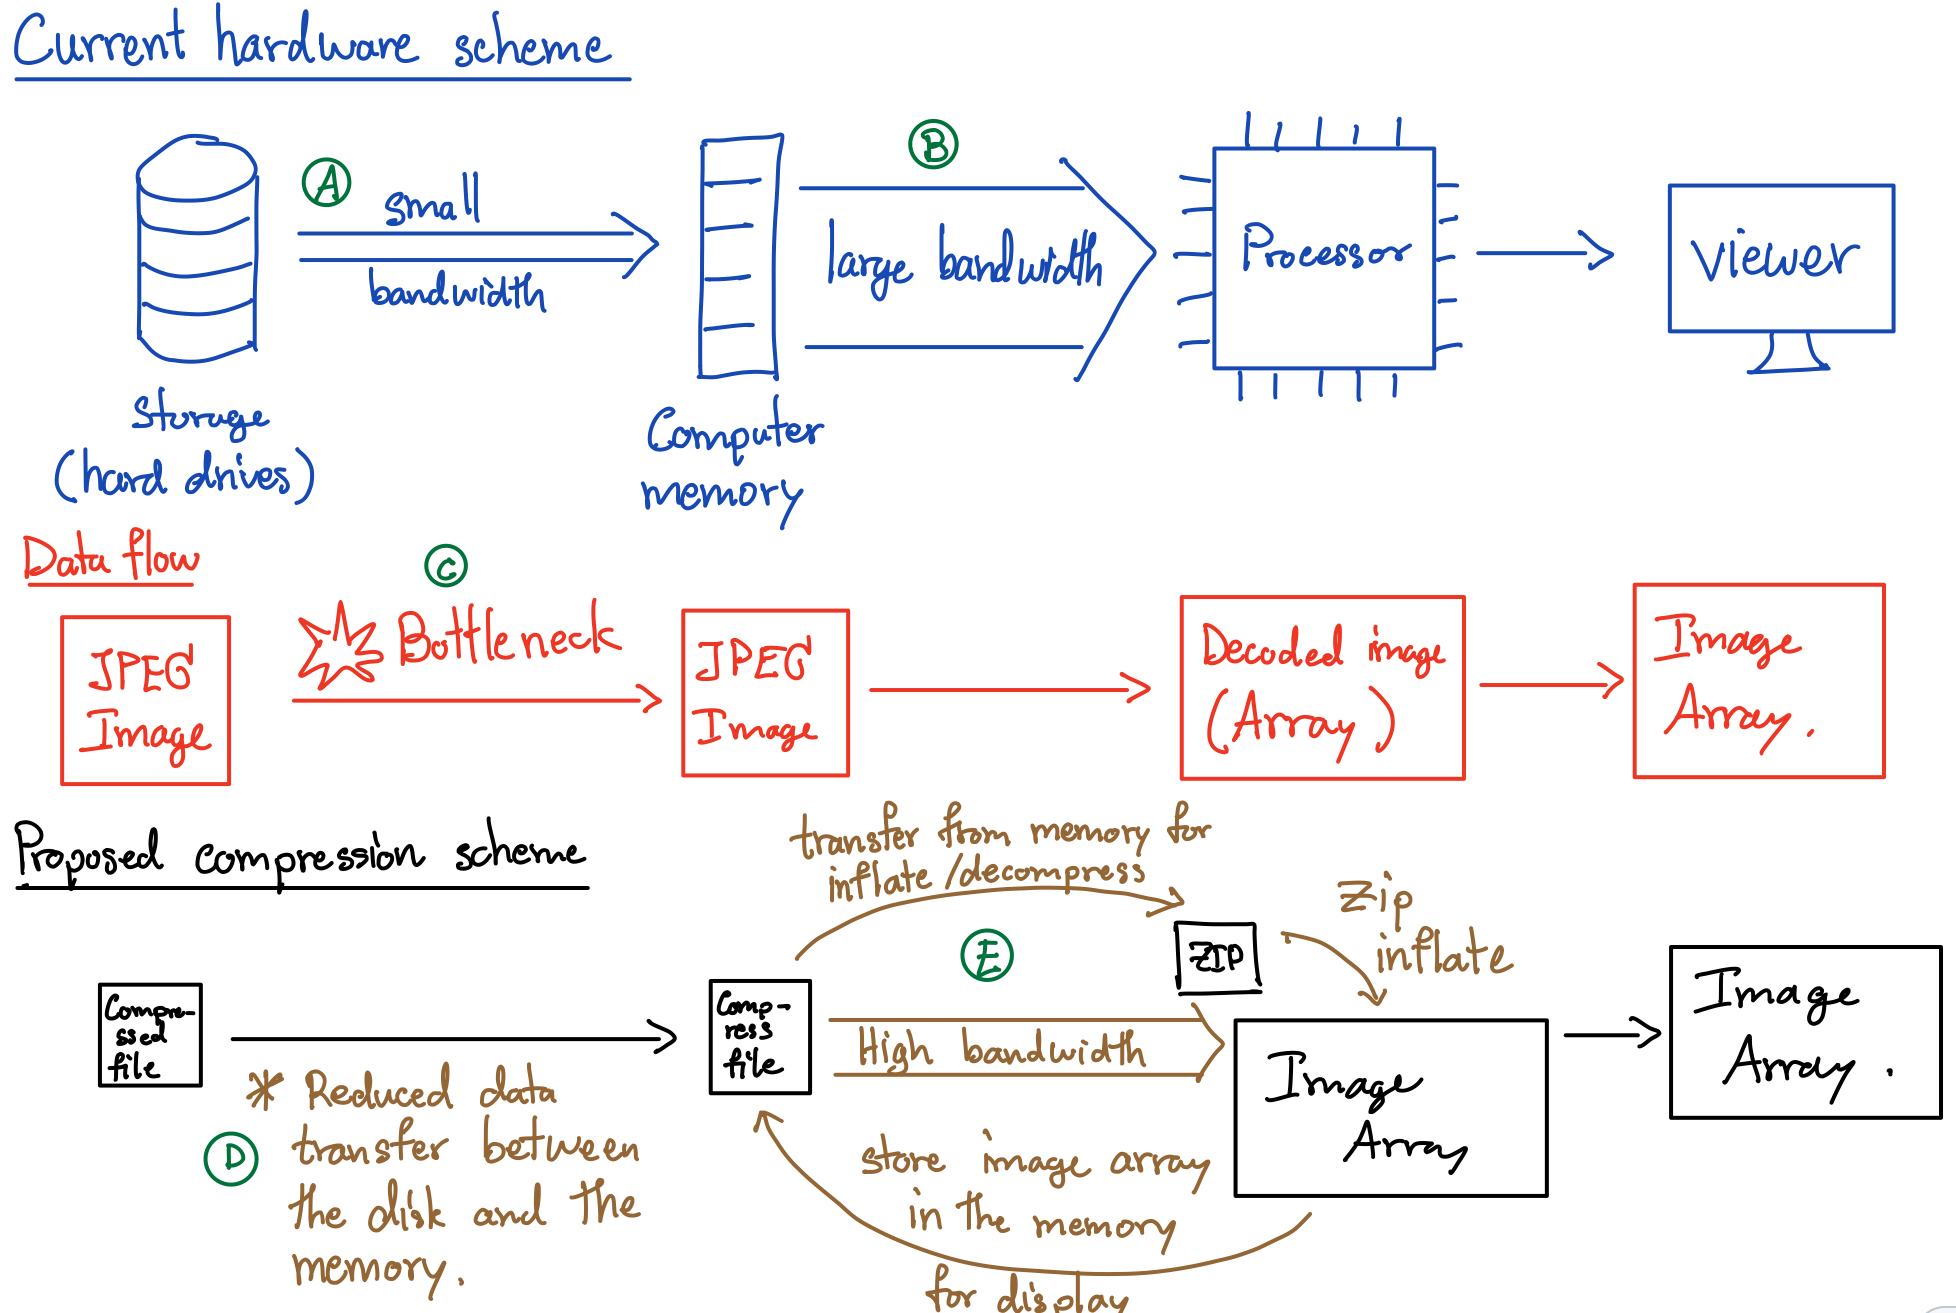
\includegraphics[width=0.9\textwidth]{proposed-scheme.jpeg}
  \caption{Networking scheme for communication protocols in digital pathology}
  \label{fig:scheme}
\end{figure}

The current processing scheme has a bottle neck. Generally, data bandwidth between a memory (RAM) and a processor is significantly higher than the one between a memory and hard drives (Fig. \ref{fig:scheme} (a-b)) and the current processing bottleneck is here (Fig. \ref{fig:scheme} (c)). My motivation is we should utilize the high memory-processor bandwidth by adopting more extensive compression algorithms. The system should read compressed file, decompress the file, and store image array (uncompressed version of the image, ready for processing). Making the final stored file as small as possible while rely on compression/decompression is the key here. Noted that I will compress each image tile, therefore we preserve ability to partially read WSIs with the proposed system. 

\subsection{Design}
The proposed system can be tested with two types of processing: (1) lossy compression and (2) lossless compression. 

In lossy compression, I will try Guetzli\footnote{\url{https://github.com/google/guetzli/}} which is a JPEG image compression algorithm from Google. It consumes more computational power, so we will test if the high-speed bandwidth between the memory and the processor can make up for it. The performance will be tested by comparing the loading or decompression speed of general JPEG files and Guetzli-compressed JPEG files. 

In lossless compression, a combination of PNG file format and DEFLATE algorithm via zlib library available natively in Python will be implemented. The reading rate will be compared. 

\subsection{Deployment and simulation results}
In deployment, the knowledge from this experiment could be applied to any of the architecture from both Paper \#1 and \#2. By reducing size of streamed data with further compression technique. 

In the experiment, one relatively small whole-slide image file was used. The file was formatted in the Aperio SVS format\footnote{\url{https://openslide.org/formats/aperio/}} \cite{Goode2013}. The file is a scanned frozen section downloaded from TCGA-KIRC project. The original file size is 22.2MB and dimension of 18,000 by 4,500 pixels which is considered to be very small piece of whole-slide scan. The origianl SVS file was converted into tiled images encoded by PNG format. Each tile has a size of 128 by 128 pixels, resulting in 4,900 tiles with total file size around 100MB. The experiment results are shown in Table \ref{tab:lossy} and \ref{tab:losless}. 


\begin{table}
    \caption{Lossy experiment}
    \centering
    \begin{tabular}{llll}
        \toprule
        Algorithm                & \multicolumn{2}{c}{Compression}  & Decompression     \\
                                 & Speed {[}sec{]} & File size      & Speed {[}sec{]}   \\
        \midrule
        Generic JPEG             &  3.7            &  13.7 MB       & 1.7               \\
        Guetzli JPEG compression &  4597           &  10.9 MB       & 1.2               \\
        \bottomrule
    \end{tabular}
    \label{tab:lossy}
\end{table}

\begin{table}[t]
 \caption{Lossless experiment}
  \centering
    \begin{tabular}{llll}
        \toprule
        Algorithm                & \multicolumn{2}{c}{Compression}  & Decompression     \\
                                 & Speed {[}sec{]} & File size      & Speed {[}sec{]}   \\
        \midrule
        Generic PNG             &  3.1            &  103 MB        & 1.4               \\
        PNG and ZLIB DEFLATE    &  7.5            &  90 MB         & 1.3 (1.1 for PNG, 0.2 for binary files) \\
        \bottomrule
    \end{tabular}
  \label{tab:losless}
\end{table}

\paragraph{Dependencies} The code for generic JPEG and PNG compression, OpenCV with OpenCV Python (v.4.1.2.30) binding was used. In JPEG compression, both quality were set to 100 (maximum value). The version of Guetzli is v1.0.1. The all related source code for all experiments in this report is made available on GitHub\footnote{\url{https://github.com/marchputt/wnmb-final-project}}. The compression experiments were tested on a computer running Ubuntu 18.4 LTS, 3.0 GHz Intel Core i7 processor, 16 GB of memory and 7200 rpm hard drive. The decompression experiments were tested on a laptop running macOS Catalina (v10.15.1), 1.7 GHz Intel Core i7 processor, 8GB or memory and SSD storage. 

\subsection{Conclusion}
\begin{itemize}
  \item Guetzli JPEG compression can generally achieve about 30\% better compression ratio resulting in 30\% smaller file size and 30\% less decompression time. 
  \item Guetzli algorithm consumes dramatically longer in compression: 1200x times longer. 
  \item The mixed PNG + zlib compression scheme can perform 10\% more efficient compression. The overall file size has been reduced, while the decompression time remains almost the same (1.3 and 1.4 seconds for mixed method and generic PNG respectively). 
  \item In the mixed compression method, DEFLATE algorithm works better in some images while PNG can achieve better compression in some other images. Examples are shown in the Figure \ref{fig:zlib-and-png}. 
  
  \begin{figure}[h]
      \centering
      \begin{tabular}{c c}
         \begin{tabular}{c c}
            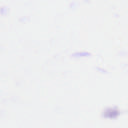
\includegraphics[width=0.18\linewidth]{z1.png}  & 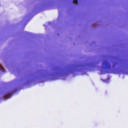
\includegraphics[width=0.18\linewidth]{z2.png} \\
            (a) & (b) \\
            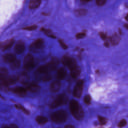
\includegraphics[width=0.18\linewidth]{z3.png}  & 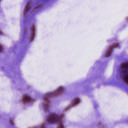
\includegraphics[width=0.18\linewidth]{z4.png} \\
            (c) & (d)
         \end{tabular} 
         
         &
         
         \begin{tabular}{c c}
            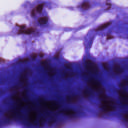
\includegraphics[width=0.18\linewidth]{p1.png}  & 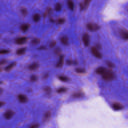
\includegraphics[width=0.18\linewidth]{p2.png} \\
            (e) & (f) \\
            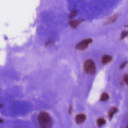
\includegraphics[width=0.18\linewidth]{p3.png}  & 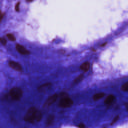
\includegraphics[width=0.18\linewidth]{p4.png} \\
            (g) & (h) 
         \end{tabular}
         
         \\
      \end{tabular}
      \caption{Comparison of images that work better with ZLIB compression (a-d) and PNG encoding (e-h). Noted that images are shown using BGR color model.}
      \label{fig:zlib-and-png}
  \end{figure}
  \item In both scheme (based on lossy and lossless compression), the file size could be reduced, therefore if we deploy this in network setting, the amount of transferring data (bandwidth amount) could be reduced from 10\% - 30\%.
  \item Currently the tile size is 128 by 128 pixels which is quite small. Compression algorithms may perform better when the tile size is bigger since they will take advantages of repeating patterns and compress them. On the other hand, once the size of tiles get bigger and the picture become more complex, compression efficiency may drop as well. Therefore, optimizing size of tiles may be necessary to improve compression efficiency. 
  \item Compression and decompression time can be improved by further code optimization. 
\end{itemize}

\bibliographystyle{unsrt}  
\bibliography{references}  %%% Remove comment to use the external .bib file (using bibtex).
%%% and comment out the ``thebibliography'' section.


% %%% Comment out this section when you \bibliography{references} is enabled.
% \begin{thebibliography}{1}

% \bibitem{kour2014real}
% George Kour and Raid Saabne.
% \newblock Real-time segmentation of on-line handwritten arabic script.
% \newblock In {\em Frontiers in Handwriting Recognition (ICFHR), 2014 14th
%   International Conference on}, pages 417--422. IEEE, 2014.

% \bibitem{kour2014fast}
% George Kour and Raid Saabne.
% \newblock Fast classification of handwritten on-line arabic characters.
% \newblock In {\em Soft Computing and Pattern Recognition (SoCPaR), 2014 6th
%   International Conference of}, pages 312--318. IEEE, 2014.

% \bibitem{hadash2018estimate}
% Guy Hadash, Einat Kermany, Boaz Carmeli, Ofer Lavi, George Kour, and Alon
%   Jacovi.
% \newblock Estimate and replace: A novel approach to integrating deep neural
%   networks with existing applications.
% \newblock {\em arXiv preprint arXiv:1804.09028}, 2018.

% \end{thebibliography}


\end{document}
